% !TEX root = ../gnss_interference_resistant_thesis.tex
\documentclass[main.tex]{subfiles}

\begin{document}

\subsection{GNSS imtuvo matavimai}

GNSS matavimai atlikti naudojant 4 HackRF imtuvus su prijungtomis
4 aktyviomis antenomis išdėstytomis kavdarto formoje $\lambda / 2$
atstumu, kaip pavaizduota \ref{fig:gnss_antenna_patern}~pav.

\begin{figure}[h]
    \begin{centering}
    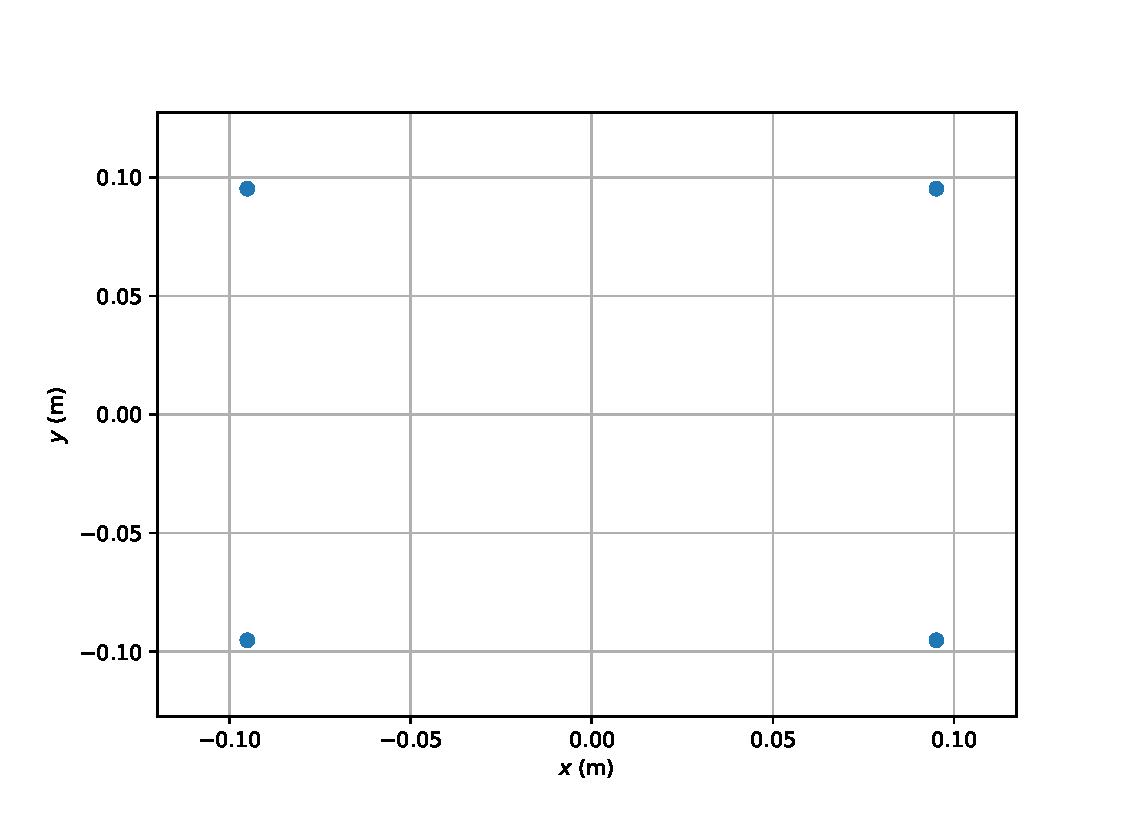
\includegraphics[scale=0.65]{drawings/antenna_pattern}
    \par\end{centering}
    \protect\caption{\label{fig:gnss_antenna_patern}Antenų masyvo, naudoto GNSS imtuvo tyrimams, išdėstymo schema.}
\end{figure}

Visi matavimai atliekami išsisaugant neapdorotus duomenų failus iš kievieno
imtuvo atskirai ir duomenų apdorojimas vykdomas šia tvarka:

\begin{enumerate}
    \item Atliekamas duomenų apdorojimas \ref{sec:gnss_doa_block} skyriuje aprašytu bloku;
    \item Atliekama fazių kalibracija pasinaudojant vienu iš matomų paldydovų;
    \item Pritaikomas MUSIC algoritmas signalų krypčių nustatymui;
    \item Duomenys apdorojami nenaudojant spindulio formavimo;
    \item Duomenys apdorojami taikant spindulio formavimo algortimą;
\end{enumerate}

\subsubsection{Fazės kalibracija naudojant GNSS signalą}

Kaip aprašyta anksteniuose skyriuose, naudojant HackRF SDR imtuvus, kiekvieno
matavimo pradžioje reikalinga fazinė imtuvų kalibracija. Tam kad supaprastinti
matavimo metodiką, fazinei kalibracijai naudojamas priimamas GPS signalas.

Tam kad būtų galima atlikti kalibracija, palydovas, pasirinktas kalibracijai,
turi būti gerai matomas, bei jis turi būti dangaus skliauto viršuje.
Kai palydovas yra statmenai antenų masyvui, visos priimamos fazės visuose
imtuvuose turi būti lygios 0. Dėl šios priežasties, matavimus reikia
planuotis iš anksto, tuo laiku kai bent vienas palydovas yra
kuo aukčiau virš horizonto. Vieno iš toliau pateiktų matavimų,
palydovų pozicijos pateiktos \ref{fig:gnss_sat_pos_calibartion}~pav.,
kalibravimui naudotas PRN29 playdovas.

\begin{figure}[ht]
    \begin{centering}
    \includegraphics[scale=1.2]{drawings/gnss_sattelites_position}
    \par\end{centering}
    \protect\caption{\label{fig:gnss_sat_pos_calibartion}GPS palydovų pozicijos dangaus skliaute, adresu Saulėtekio al. 9, Vilnius, 2022-05-11 13:20.}
\end{figure}

Kalibracija atliekama lyginant vienos iš antenų fazę, su kitų trijų antenų fazėmis.
Atliekamas vidurkio skaičiavimas, gauta vertė atitinka fazės nuokrypį nuo tikrosios
fazės, ši vertė naudojama fazės pastumimui visuose skaičiavimuose.

Jeigu palydovas nėra statmenas antenų masyvui, pritaikius spindulio formavimo
algoritmą, galime suskaičiuoti fazes kiekvienoje antenoje ir šis pokrypis
yra pridedamas prie nulinės fazės. Fazių kalibracijos pavyzdys pateiktas
\ref{fig:gnss_phase_calibration}~pav.

\begin{figure}[ht]
    \begin{centering}
    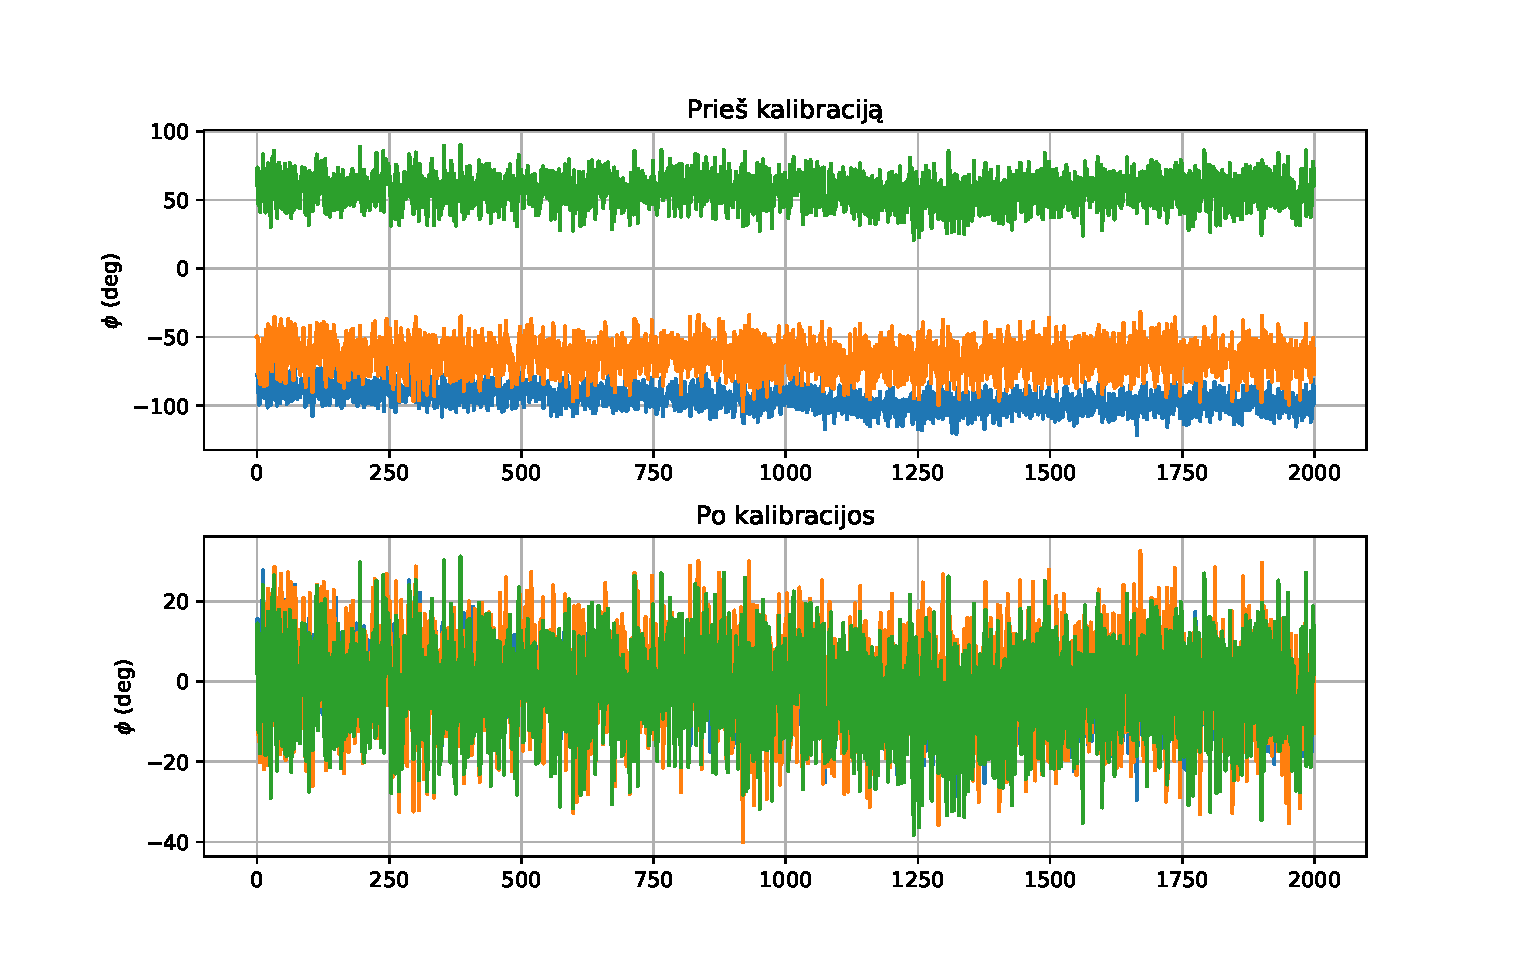
\includegraphics[scale=0.65]{drawings/phase_calibration}
    \par\end{centering}
    \protect\caption{\label{fig:gnss_phase_calibration}PRN29 playdovo priimto signalo fazės kiekviename antenų masyvo elemente, prieš kalibraciją ir po kalibracijos.}
\end{figure}


\subsubsection{GNSS signalų priėmimas kai atspindžiai vyksto nuo vieno pastato}

\begin{figure}[ht]
    \begin{centering}
    \includegraphics[scale=0.45]{drawings/one_reflection_2}
    \par\end{centering}
    \protect\caption{\label{fig:single_reflection}Nustatytos GPS palydovų signalų kryptys, naudojant MUSIC algoritmą.}
\end{figure}

\begin{figure}[ht]
    \begin{centering}
    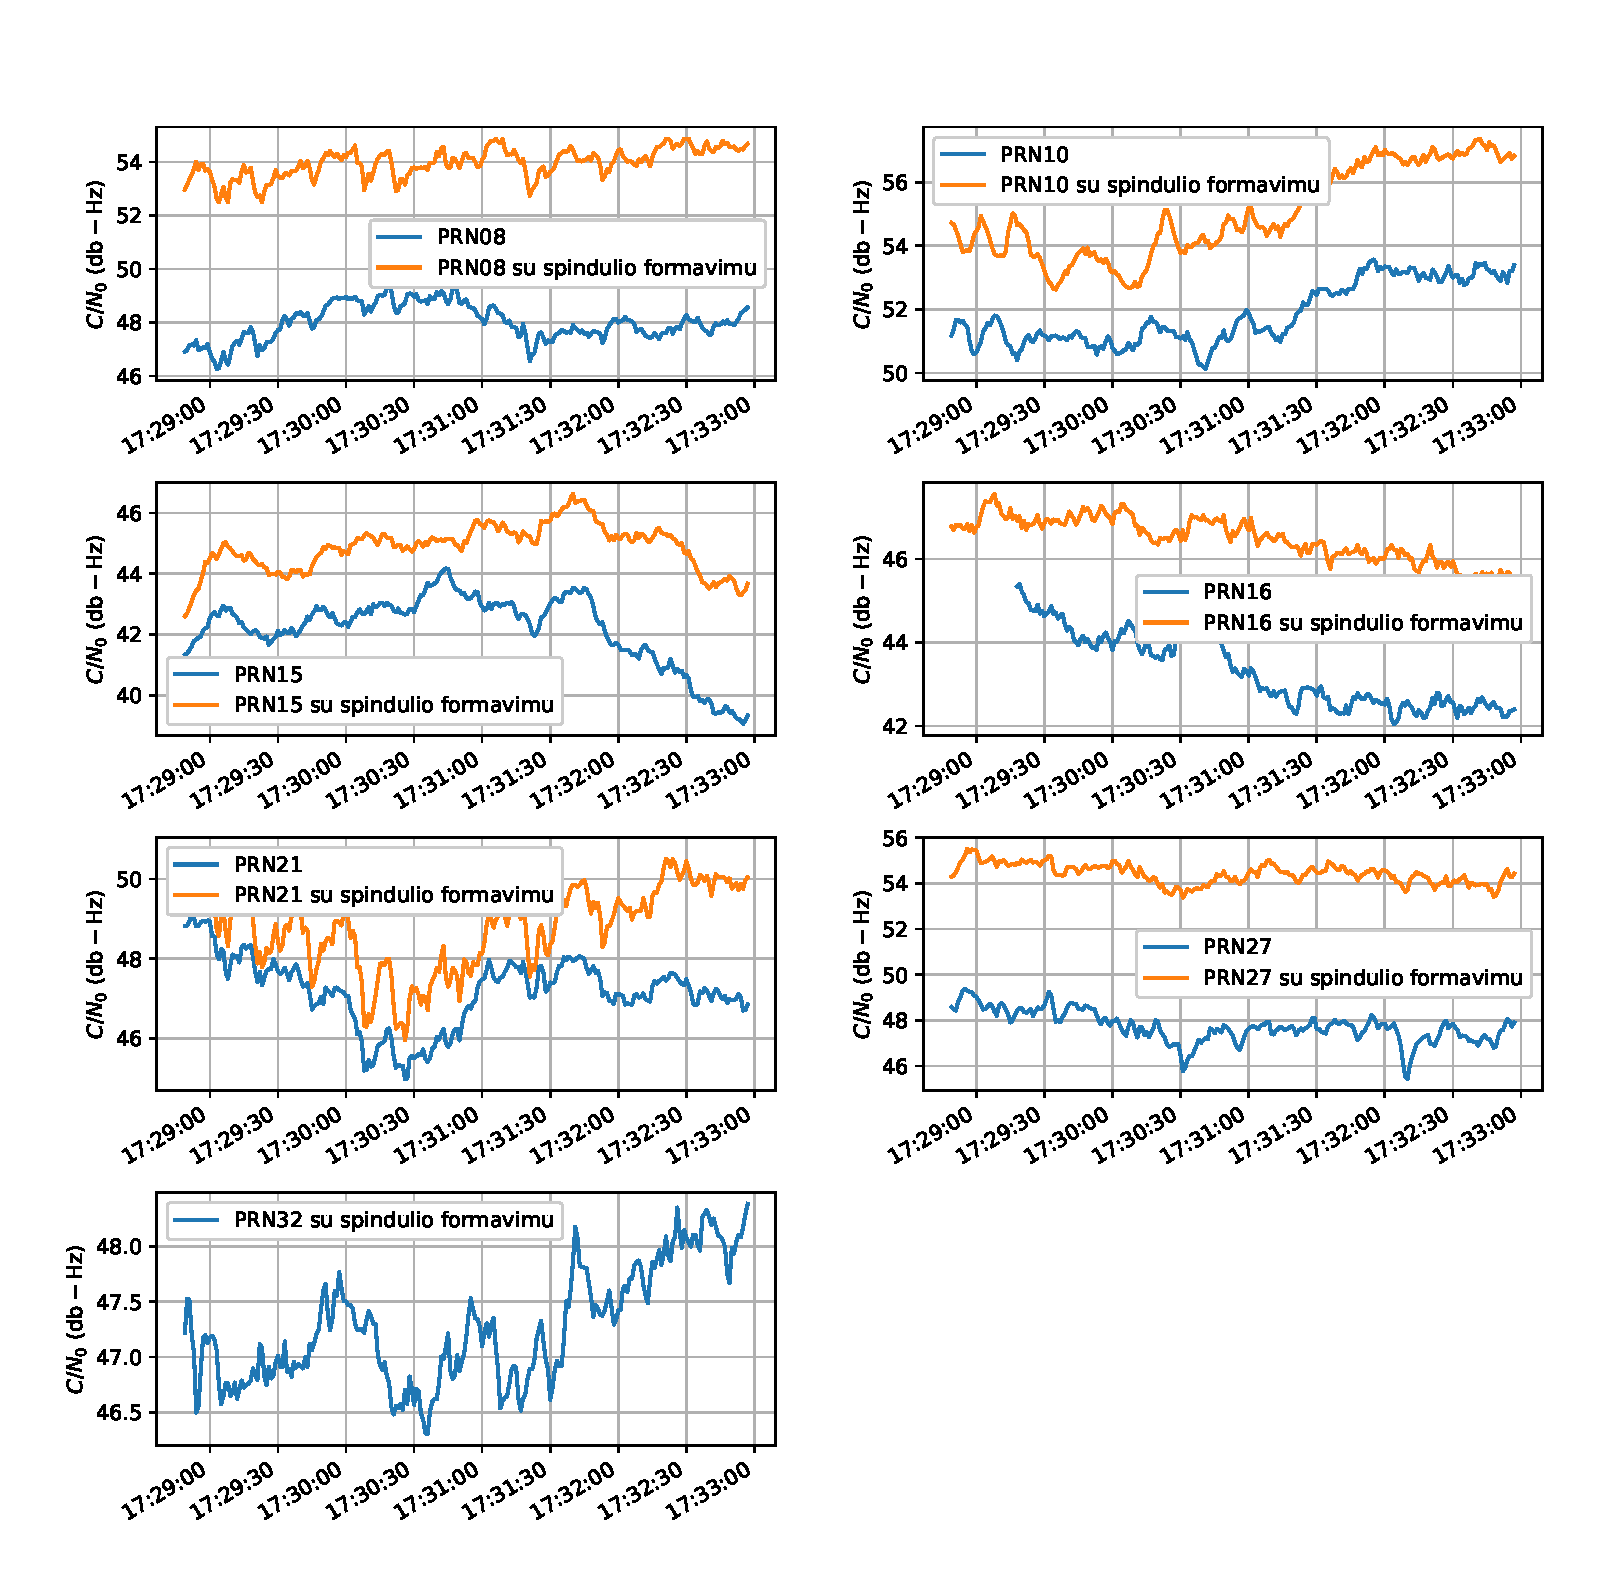
\includegraphics[scale=0.6]{drawings/one_reflection_snr}
    \par\end{centering}
    \protect\caption{\label{fig:single_reflection_snr}Nustatytas signalo triukšmo santykys nenaudojant ir naudojant spindulio formavimą.}
\end{figure}

\begin{figure}[ht]
    \begin{centering}
    \hspace*{-4cm}\includegraphics[scale=0.5]{drawings/one_reflection_map}
    \par\end{centering}
    \protect\caption{\label{fig:single_reflection_map}Imtuvo pozicijos koordinatės su spindulio formavimu ir be spindulio formavimo. Žemėlpis \cite{google_maps}.}
\end{figure}

\end{document}
